\documentclass{article}
\usepackage{graphicx}
\usepackage{hyperref}
\usepackage{caption}
\usepackage{subcaption}
\usepackage{mathtools}
\usepackage[dutch]{babel}

\begin{document}

\begin{center}
	\huge{Wiskunde in Kunst}\\
	\LARGE{Opdracht 10} \\
	
	\vspace{2cm}
	
	\Large{Fractals en de Gulden Snede}\\
	
	\vfill
	
	\begin{figure}[Hh]
		\centering
		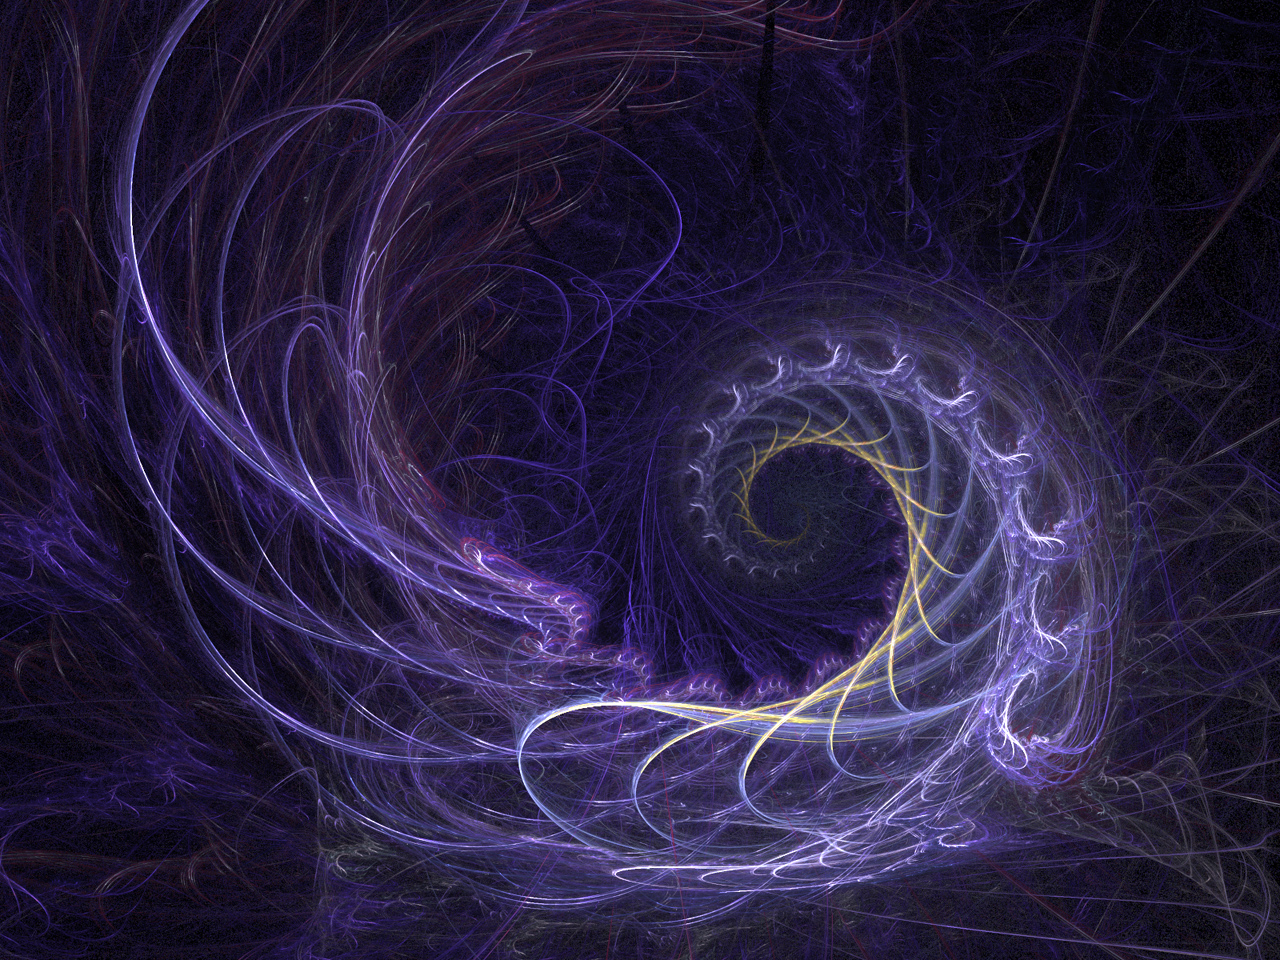
\includegraphics[width=\textwidth]{Golden_Ratio.jpg}
	\end{figure}
	
	\vfill
	\Large{Marcelo Dias Avelino} \hfill \large{0840416}
\end{center}

\thispagestyle{empty} % Remove page numbering

\pagebreak

\setcounter{page}{1} % Start counting pages here

\section{De relatie}

Zoals uitgelegd in de vorige verslagen, een fractal is een figuur die opgebouwd is uit delen dat min of meer gelijk zijn aan het algemene figuur. Fractals hebben oneindig veel detailles en kunnen oneindig worden ingezoomd zonder enige detail te verliezen. Ze zijn opgebouwd uit een verzameling regels en waardes en \'e\'en van de veel voorkomende waardes is de gulden snede. Een voorbeeld hiervan is de Fibonacci spiraal die eerder opgenoemd is in andere opdrachten en afgebeeld is in Figuur \ref{fig:spiral}. Dit is een spiraal die opgebouwd is uit de bekende Fibonacci reeks en deze reeks volgt een simpele regel: een getal is een opsomming van de twee voorgaande getallen. Als \'e\'en van deze getallen door de voorgaande getal zal dit in de buurt van de gulden snede uitkomen. Verder is deze spiraal is een fractal omdat het niet uitmaakt hoever er in gezoomd of uit gezoomd wordt, het zal altijd ongeveer hetzelfde uitzien. 

\begin{figure}[Hh]
	\centering
	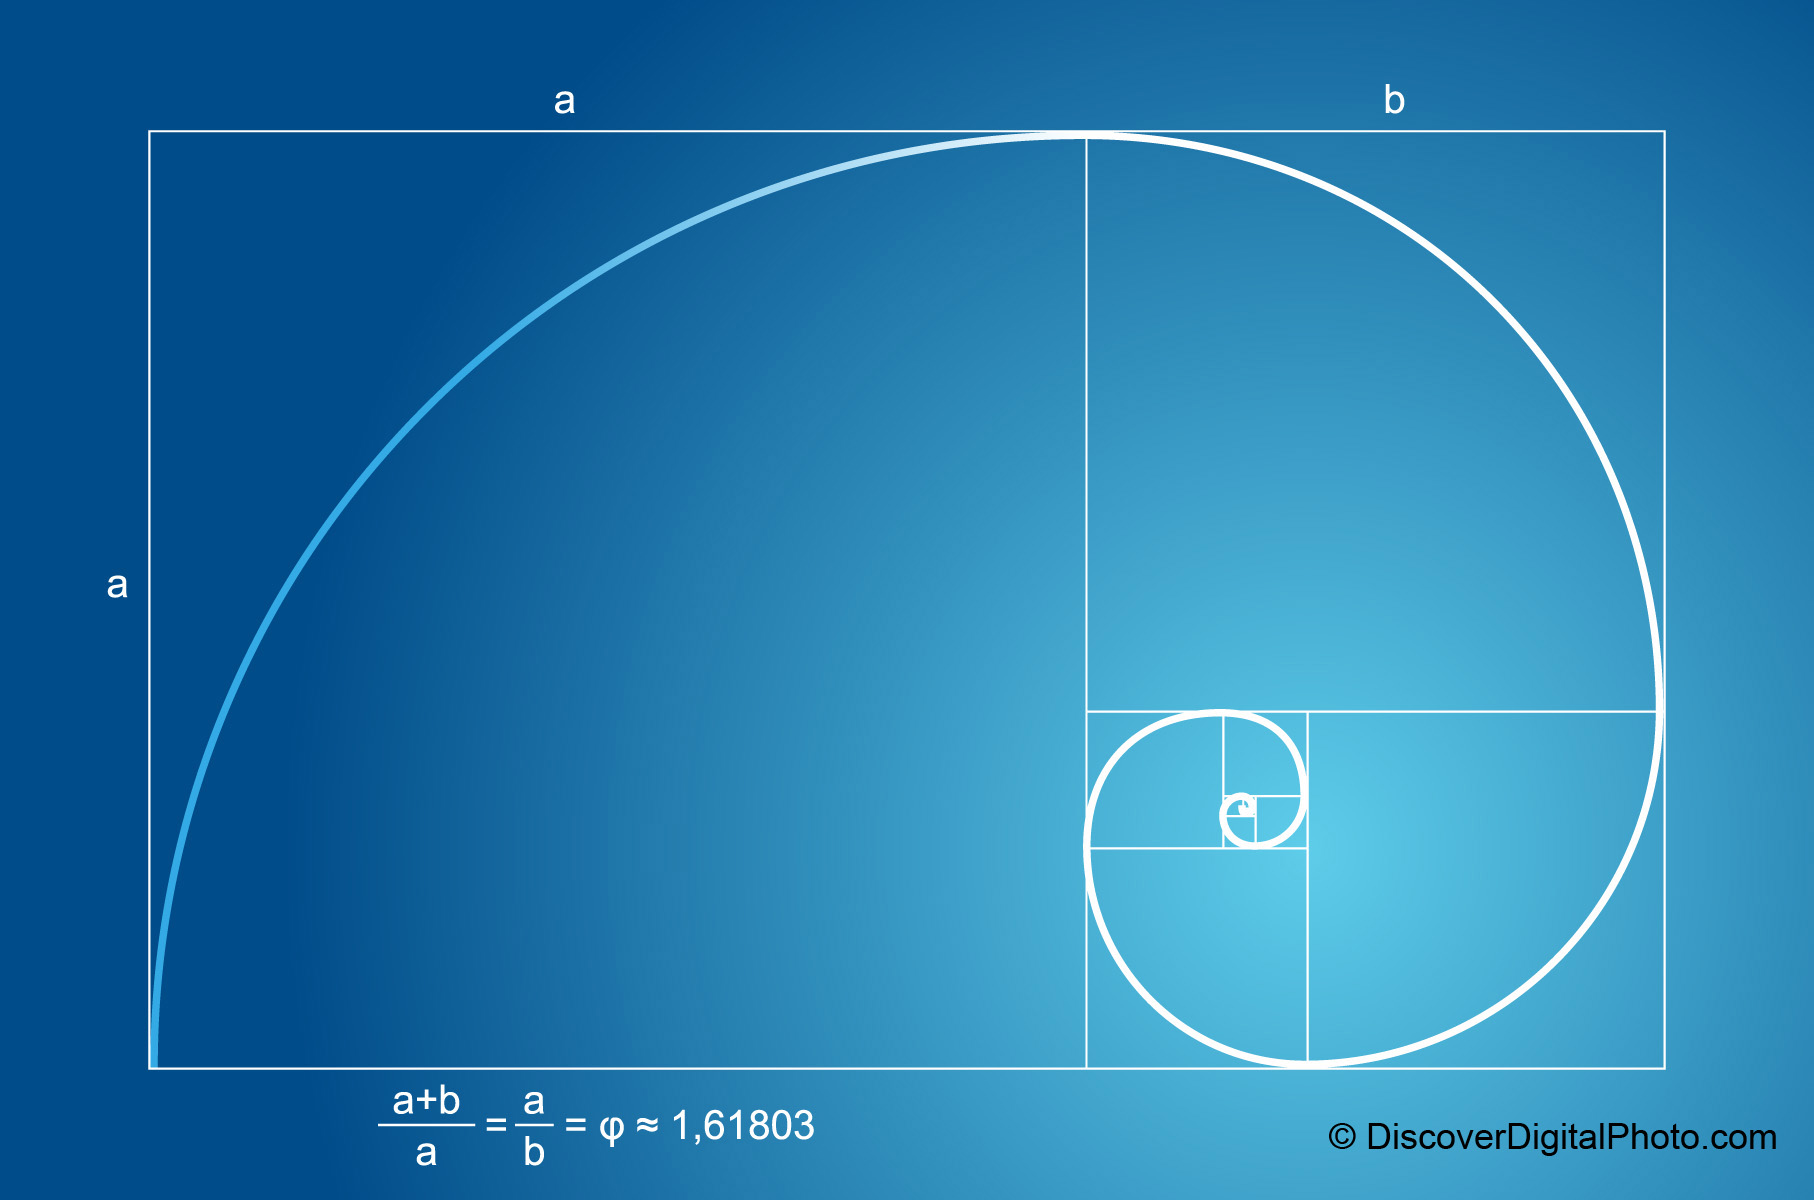
\includegraphics[width=0.6\textwidth]{fibonacci_good1.jpg}
	\caption{De Fibonacci spiraal.}
	\label{fig:spiral}
\end{figure}

Een tweede voorbeeld komt eigenlijk weer terug op de Fibonacci reeks. In dit voorbeeld is de Mandelbrot fractal aan de buurt, die te zien is in Figuur \ref{fig:mandlebrot}. Hier kunnen de aantal uitsteeksels op worden geteld van elke `bol'. Hieruit blijkt heel snel dat ook de Mandlebrot fractal gebaseerd is op de gulden snede.

\begin{figure}[Hh]
	\centering
	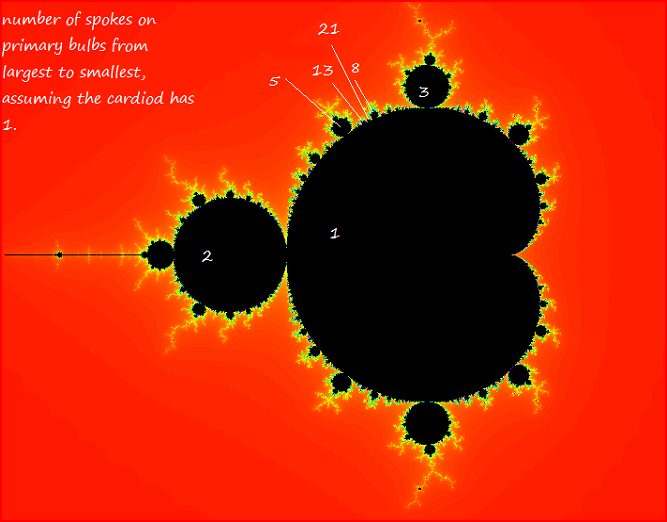
\includegraphics[width=0.7\textwidth]{mandlebrot5.png}
	\caption{Madelbrot fractal.}
	\label{fig:mandlebrot}
\end{figure}

\end{document}
